\documentclass{article}

\usepackage[margin=3cm]{geometry}
\usepackage{amsmath}
\usepackage{amsfonts}
\usepackage{amssymb}
\usepackage{amscd}
\usepackage{standalone}
\usepackage{float}
\usepackage{color}
\usepackage[shortlabels]{enumitem}
\usepackage{graphicx}
\usepackage{caption}
\usepackage[ngerman]{babel}
\usepackage{lscape}
\usepackage{cancel}
\usepackage{dirtytalk}
\usepackage{siunitx}
\usepackage[style=numeric,backend=biber,sorting=none]{biblatex}

\graphicspath{ {./images/} }
\addbibresource{references.bib}

\begin{document}
\begin{titlepage}
    \centering
    {\scshape\LARGE Hochschule für Technik und Wirtschaft Dresden \par}
    \vspace{1cm}
    {\scshape\Large Beleg \glqq Computergrafik I\grqq\par}
    \vspace{1.5cm}
    {\huge\bfseries Dokumentation\par}
    \vspace{2cm}
    {\Large\itshape Raphael Neubert \par}
    \vfill
    \begin{minipage}{0.3\textwidth}
        Studiengang:\\
        Studiengruppe:\\
        Matrikelnummer:
    \end{minipage}
    \begin{minipage}{0.3\textwidth}
        Informatik\\
        20/041/61\\
        49916
    \end{minipage}
    \vfill

    {\large \today\par}
\end{titlepage}
\tableofcontents
\newpage

\section{Aufgabenbeschreibung}
Aufgabe der Belegarbeit ist es ein Programm zu schreiben, welches eine interaktive, zeitlich animierte Szene
mit mehreren dreidimensionalen Objekten, enthält. Die Objekte unterscheiden sich dabei in ihrer Form und Farbe
bzw. ihrer Textur. Die Objekte sollen dann durch verschiedenartigen Lichtquellen beleuchtet werden so, dass
auf den Objekten die unterschiedlichen Beleuchtungseffekte sichtbar werden. Das Ergebnis soll anschließend
gleichzeitig in mehreren Viewports, die verschiedene Ansichten und Projektionen zeigen, dargestellt werden.
Zur Entwicklung soll die Programmiersprache C++ mit den Bibliotheken freeglut, glew, freeimage und glm genommen werden.
Das Ergebnis dieser Aufgabe soll zum Schluss als Visual-Studio-C/C++ Projekt, sowie in ausführbarer Form
als exe-Datei, vorliegen.
\section{Vorgehensweise}\label{Vorgehensweise}
Zu Beginn meiner Bearbeitung der Belegarbeit habe ich mich intensiv mit der Aufgabenstellung beschäftigt und Ideen
für die konkrete Umsetzung gesammelt. Anschließend habe ich überlegt welche meiner Ideen, in der Umsetzung mit meinem
Wissensstand und der, aufgrund vieler anderer Belegarbeiten, doch recht knappen Zeit, machbar sind.
Nach den notwendigen Überlegungen traf ich dann eine Entscheidung.\par
\medskip
Ich wollte eine Szene Programmieren in der man mich frei bewegen kann. Die Steuerung sollte dabei der eines
Computerspiels ähneln. Als Objekte entschloss ich mich einen Würfel und einen Kegel zu nehmen wobei sich die
Texturierung der beiden Objektarten unterscheidet. Von den Objekten wollte ich dann sehr viele Instanzen erzeugen und diese
sich in ihrer Position zeitlich verändern lassen. Als Lichtquellen entschloss ich mich eine art Lichtwürfel, ähnlich einer
Sonne mit dem Unterschied das eine Sonne ein direktionales, der Würfel aber ein positionelles Licht, ist und eine
art Taschenlampe, zu nehmen. Bei den Viewports entschloss ich mich für vier Verschiedene. Der Erste mit einer realistischen, 
perspektivischen Ansicht, der Zweite mit einer orthogonalen Seitenansicht, der Dritte mit einer orthogonalen
Draufsicht und der vierte mit einer weiteren orthogonalen Ansicht dessen Betrachtungswinkel abhängig von der Mausposition ist.
Ich nahm mir auch vor einige durch Tastaturevents veränderbare Einstellungen zu implementieren die Auswirkungen auf die
Ansicht, die Lichtfarbe oder andere Effekte haben.\par
\medskip
Entwickelt habe ich mein Programm auf einem Linux Betriebssystem. Erst nach dem das Programm fertig war habe ich es
mit Visual-Studio geöffnet und die notwendigen Veränderungen vorgenommen um es auf Windows lauffähig zu bekommen.
Zur Versionierung verwendete ich Git und ein privates Repository auf Github.\par
\medskip
Am Anfang der Entwicklung entschloss ich mich keine meiner bisher in den Praktika verwendeten Funktionen zu verwenden
sondern von Null anzufangen. Deshalb entwickelte ich zunächst eine Klasse \say{Shader} welche mir eine einfache
Handhabung von verschiedenen Shaderprogrammen ermöglicht. Dazu gehört das Compilieren und
Aktivieren von Shadern sowie das setzen von uniform Variablen. Anschließend entwickelte ich die Klasse \say{Camera} welche
für die Berechnung der \say{View}-Matrizen dient. Die Inhalte der Klassen orientierte ich großteils an meinen im Praktikum
verwendeten prozeduralen Implementierungen. Anschließend erstellte ich eine \say{main} Datei und füllte sie mit einem
Grundgerüst für ein OpenGL Programm.\par
\medskip
Nach der Entwicklung der wichtigsten Grundabstraktionen entwickelte ich Funktionen zur Generierung und Zeichnung
der gewählten Objekte: Würfel und Kegel. Ich entschloss mich dabei indiziertes Zeichnen zu verwenden um Redundanzen zu
vermeiden. Auf Texturkoordinaten sowie Normalenvektoren verzichtete ich zunächst. Als nächstes schrieb ich eine
Funktion die Objekte im Raum abhängig von der Zeit anordnet und die Instanzen dieser Objekte, in Form eines \say{structs}
in dem sich ein Array für die Modelmatrizen der Würfel und eines für die Modelmatrizen der Kegel befindet, speichert.
Die Würfel werden in einem Quadrat angeordnet wobei die $y$-Position abhängig von der Zeit und der $x,y$-Position des
Würfels im Quadrat. Um eine art Verlauf zu bekommen verwendete ich verschiedene trigonometrische Funktionen.
In jeder fünften Spalte wird in jeder fünften Reihe des Quadrats auf einem Würfel ein Kegel platziert
die $y$-Position des Kegels verändert sich dabei genau so wie die von dem Würfel auf dem der Kegel steht.
Ich entschloss mich anschließend eine sehr große Anzahl an Objekten zu generieren. Die dadurch notwendige Optimierung
ist unter 6.n beschrieben. Nach dem Platztieren der Objekte entschloss ich mich das es ein guter Zeitpunkt ist 
den Objekten Texturen zu geben. Nach der Texturierung begann ich an verschiedenen Lichtquellen zu arbeiten.
Ich fügte den Objekten Normalenvektoren hinzu und entwickelte Fragmentshader welche die Farbe eines Fragmentes
abhängig von dem Winkel (Normalenvektor) zur Lichtquelle, der Entfernung und dem Winkel von Objekt zur Kamera berechnet.
Des weiteren platzierte ich einen Würfel im Raum von dem das Licht auszugehen scheint.
Auf ähnliche Art und Weise programmierte ich dann eine Taschenlampe.
Dabei ist die Position der Lichtquelle gleich der Position der Kamera. Der Lichtkegel der 
Taschenlampe entsteht durch Verdunklung von Fragmenten deren Winkel zur Lichtquelle (Kamera) größer als der Öffnungswinkel
der Taschenlampe ist. Nach der Implementierung des Lichts entwickelte ich einige Einstellungen die sich durch
Tastaturevents verändern lassen. Dazu gehört die Ansicht, die Farbe des Lichts, die Art des Lichts
(Lichtwürfel oder Taschenlampen) und Änderung von OpenGL Einstellungen wie zum Beispiel Face Culling oder der Tiefentest.
Zu letzt implementierte ich die verschiedenen Viewports.
\section{Installation}
\subsection{Windows}
\subsection{Linux}
\newpage
\section{Bedienung}
\subsection{Kamera}
Die Steuerung der Kamera ähnelt der eines Computerspiels. Deshalb werden die Pfeiltasten durch die Tasten \textit{w,a,s,d}
ersetzt.
\begin{figure}[H]
    \centering
    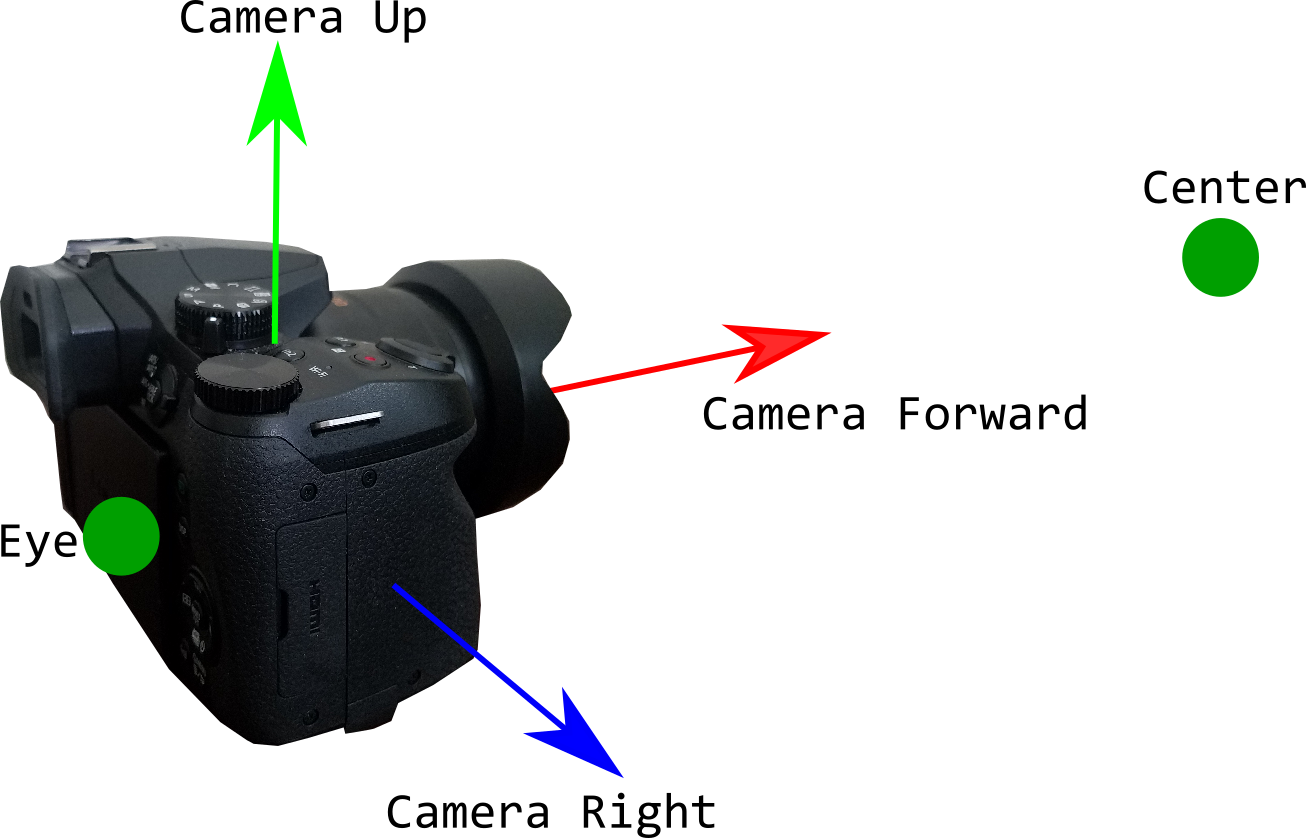
\includegraphics[scale=0.231]{camera.png}
\end{figure}
\subsubsection{Tastatur}
\begin{table}[H]
    \begin{tabular}{|l|l|p{100mm}|}
\hline
\textit{\textbf{Taste}} & \textit{\textbf{Vergleich}} & \textit{\textbf{Beschreibung}}\\ \hline
\textbf{w}              & nach vorne bewegen          & Verschiebung der Kamera entlang des Blickrichtungsvektors
(im Bild \say{Forward}).\\ \hline
\textbf{a} & nach links bewegen  & Verschiebung der Kamera entlang des Gegenvektors vom Vektor
der nach Rechts zeigt (im Bild \say{Right}).\\ \hline
\textbf{s} & nach hinten bewegen & Verschiebung der Kamera entlang des Gegenvektors vom Blickrichtungsvektor.\\ \hline
\textbf{d}              & nach rechts bewegen         & Verschiebung der Kamera entlang des Vektors
der nach Rechts zeigt.\\ \hline
\textbf{e}              & nach oben bewegen           & Verschiebung der Kamera entlang des Vektors
der nach oben zeigt (im Bild \say{Up}).\\ \hline
\textbf{q} & nach unten bewegen  & Verschiebung der Kamera entlang des Gegenvektors vom Vektor
der nach oben zeigt.   \\ \hline
\end{tabular}
\end{table}
\subsubsection{Maus}
\begin{table}[H]
    \begin{tabular}{|l|l|p{74mm}|}
\hline
\textit{\textbf{Mausbewegung}} & \textit{\textbf{Vergleich}} & \textit{\textbf{Beschreibung}}\\ \hline
\textbf{nach links}            & Kamera nach links drehen    & Linksdrehung entlang des Vektors der nach oben zeigt.\\ \hline
\textbf{nach rechts} & Kamera nach rechts drehen & Rechtsdrehung entlang des Vektors der nach oben zeigt.  \\ \hline
\textbf{nach oben}             & Kamera nach oben neigen     & Rechtsdrehung entlang des Vektors
der nach rechts zeigt. Um eine einfachere Orientierung zu ermöglichen kann der Rotationswinkel maximal
\ang{89} erreichen.\\ \hline
\textbf{nach unten}  & Kamera noch unten neigen  & Linksdrehung entlang des Vektors der nach rechts zeigt.
Der Rotationswinkel kann in diese Richtung nicht kleiner als \ang{-89} werden.\\ \hline
\end{tabular}
\end{table}
\subsection{Licht}
\subsubsection{Lichtquelle}
Die Art der Lichtquelle kann durch Betätigung der Taste \say{\textit{l}} zwischen einem \say{Lichtwürfel} und einer
Taschenlampe gewechselt werden.\\
\begin{minipage}{0.55\textwidth}
\begin{figure}[H]
    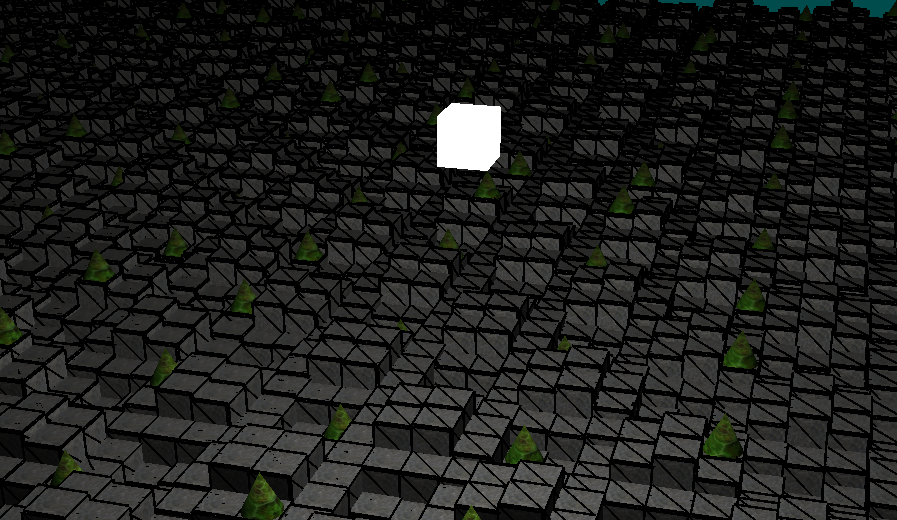
\includegraphics[scale=0.258]{lmode1.png}
    \caption{Lichtwürfel}
\end{figure}
\end{minipage}
\begin{minipage}{0.45\textwidth}
\begin{figure}[H]
    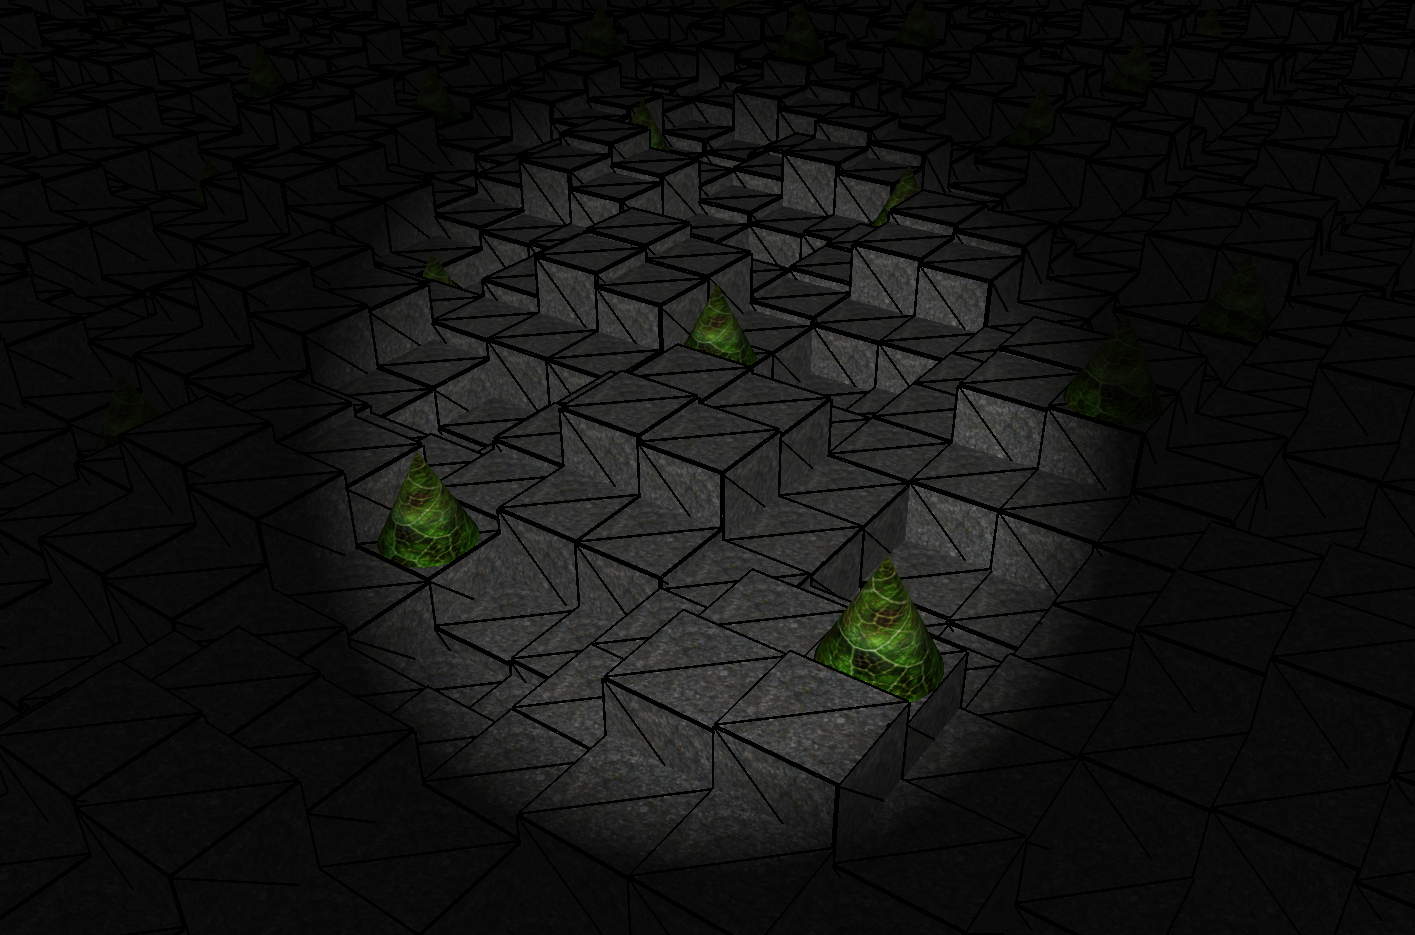
\includegraphics[scale=0.145]{lmode2.png}
    \caption{Taschenlampe}
\end{figure}
\end{minipage}

\subsubsection{Lichtfarbe}
Die Farbe des Lichtes kann mit der Taste \say{\textit{c}} zwischen weiß, rosa, blau und rot verändert werden.
Dies funktioniert sowohl bei dem Lichtwürfel als auch bei der Taschenlampe.\\
\begin{minipage}{0.5\textwidth}
\begin{minipage}{0.485\textwidth}
\begin{figure}[H]
    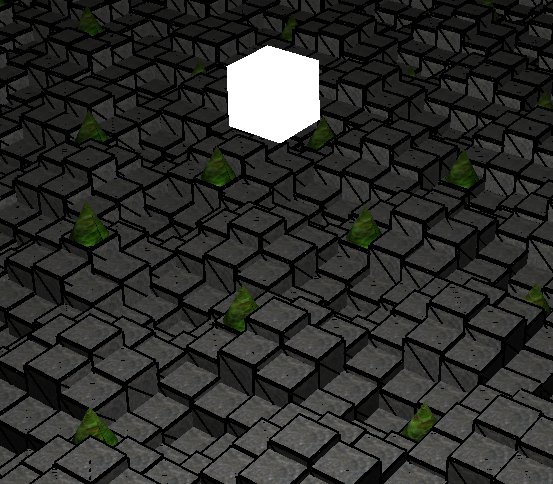
\includegraphics[scale=0.2]{lcolor1.png}
    \caption{weiß}
\end{figure}
\end{minipage}
\begin{minipage}{0.25\textwidth}
\begin{figure}[H]
    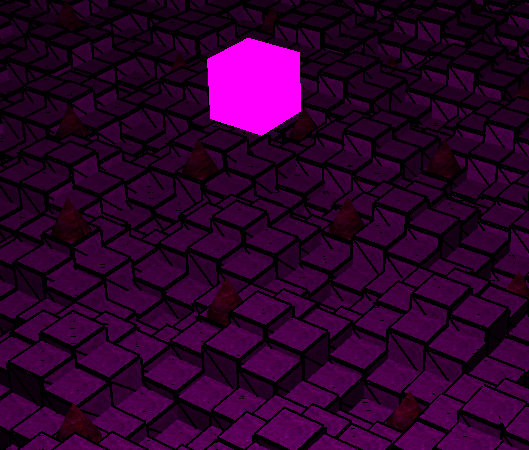
\includegraphics[scale=0.215]{lcolor2.png}
    \caption{rosa}
\end{figure}
\end{minipage}
\end{minipage}
\begin{minipage}{0.5\textwidth}
\begin{minipage}{0.49\textwidth}
\begin{figure}[H]
    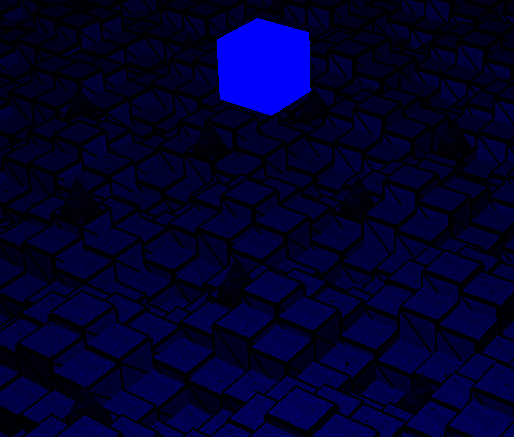
\includegraphics[scale=0.221]{lcolor3.png}
    \caption{blau}
\end{figure}
\end{minipage}
\begin{minipage}{0.25\textwidth}
\begin{figure}[H]
    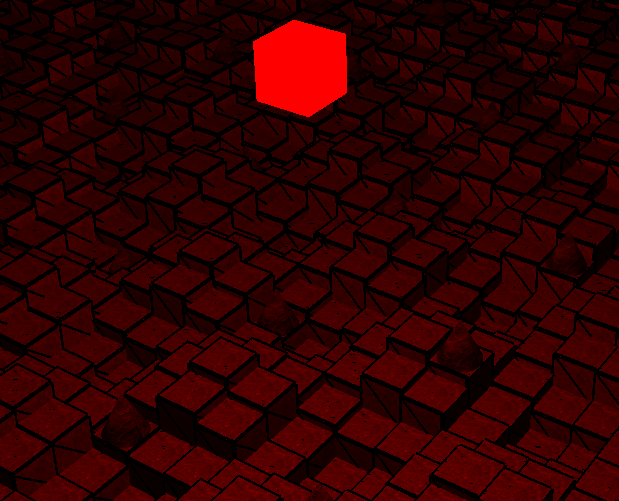
\includegraphics[scale=0.192]{lcolor4.png}
    \caption{rot}
\end{figure}
\end{minipage}
\end{minipage}

\subsection{Viewports}
Standardmässig wird nur ein einziger Viewport, der so groß wie das Fenster des Programmes ist und eine realistische,
perspektivische Ansicht darstellt. Dies vereinfacht das erlernen der Steuerung der Kamera
und Endecken der Szene. Durch Betätigung der Taste \say{\textit{v}} lässt sich die Ansicht in einen Modus
mit vier Viewports versetzen.
\begin{table}[H]
\begin{tabular}{|l|l|}
\hline
\textit{\textbf{Position}} & \textit{\textbf{Ansicht}}   \\ \hline
\textbf{unten links}       & realistisch, perspektivisch \\ \hline
\textbf{unten rechts}      & orthogonale Seitenansicht   \\ \hline
\textbf{oben links}        & orthogonale Draufsicht      \\ \hline
\textbf{oben rechts} & orthogonale Ansicht,  Betrachtungswinkel ist von Mausbewegung abhängig \\ \hline
\end{tabular}
\end{table}

\begin{minipage}{0.5\textwidth}
\begin{figure}[H]
    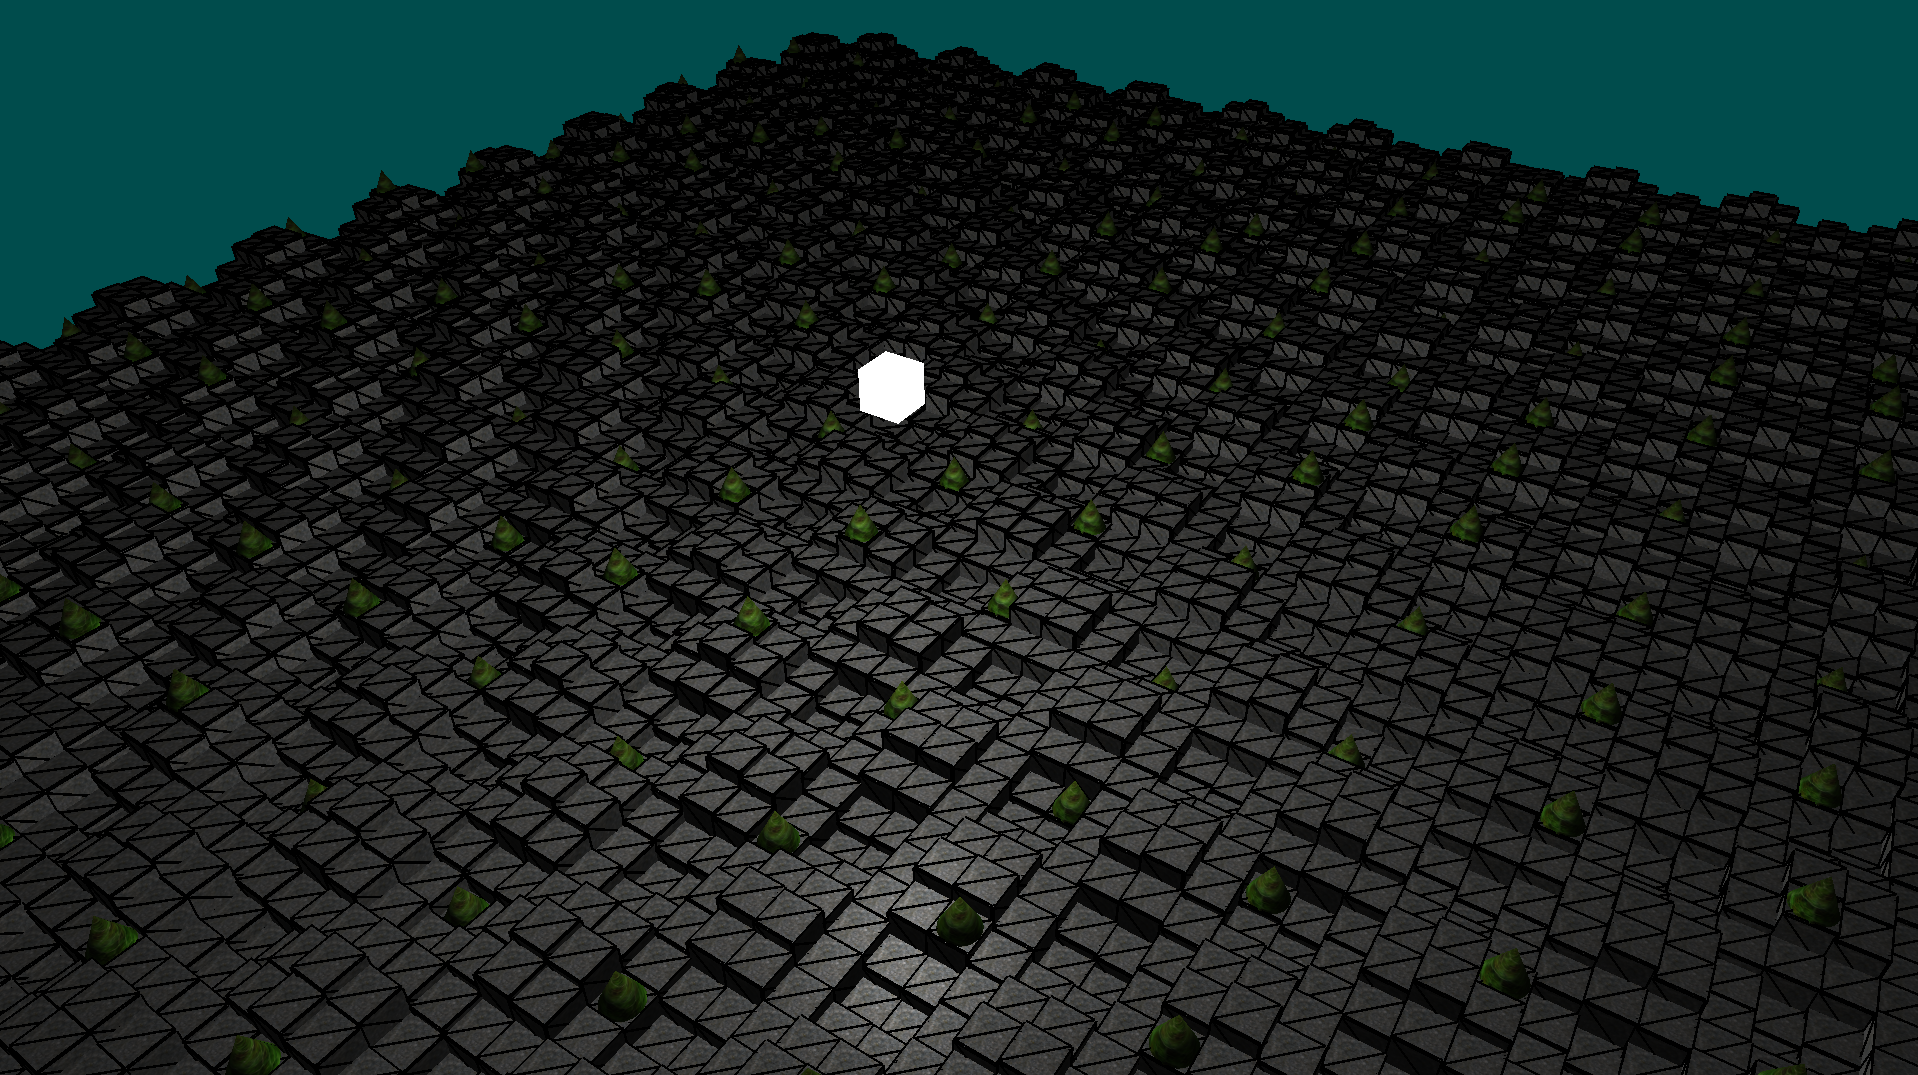
\includegraphics[scale=0.12]{vmode1.png}
    \caption{einzelner Viewport}
\end{figure}
\end{minipage}
\begin{minipage}{0.5\textwidth}
\begin{figure}[H]
    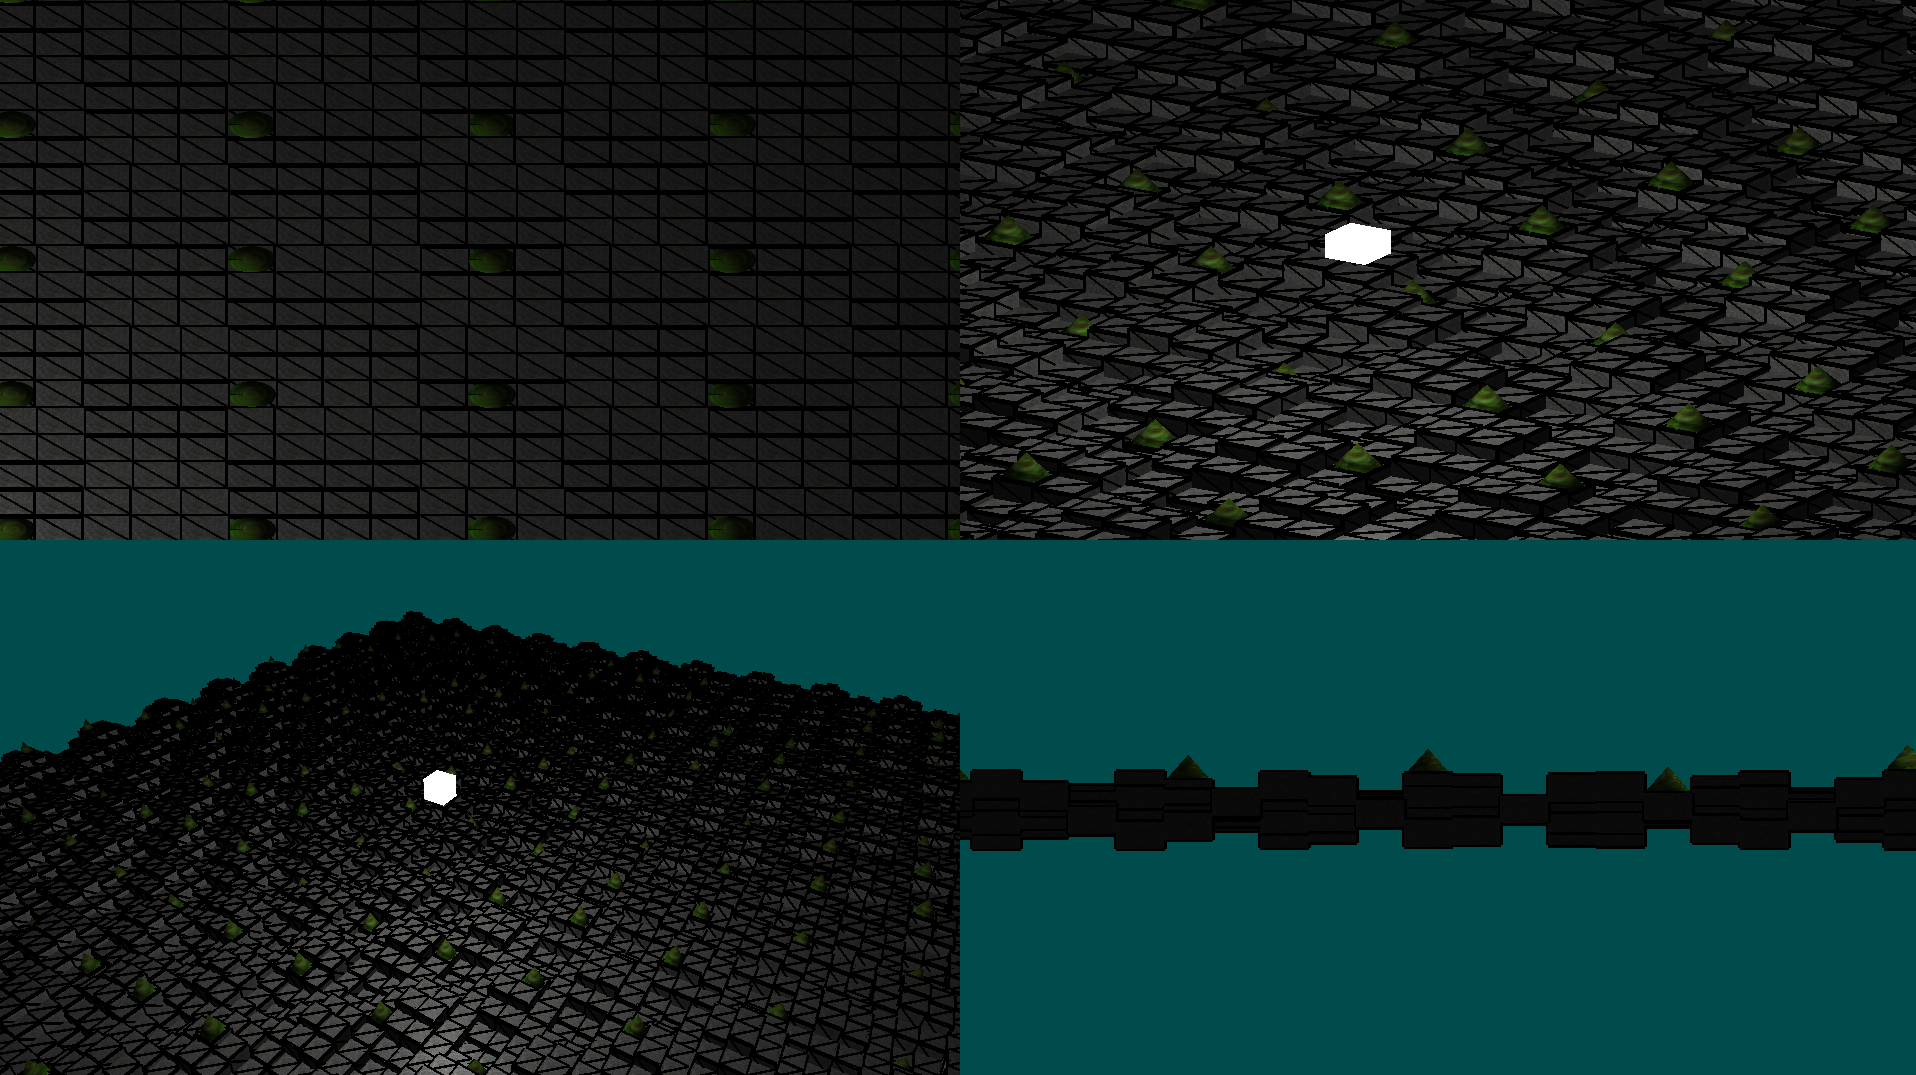
\includegraphics[scale=0.12]{vmode2.png}
    \caption{vier Viewports}
\end{figure}
\end{minipage}

\subsection{Wireframe Modien}
Mit der Taste \say{\textit{m}} lässt sich zwischen 5 verschiedenen Modien wechseln welche entscheiden ob und wie
die Wireframes angezeigt werden.\\
\begin{minipage}{0.5\textwidth}
\begin{figure}[H]
    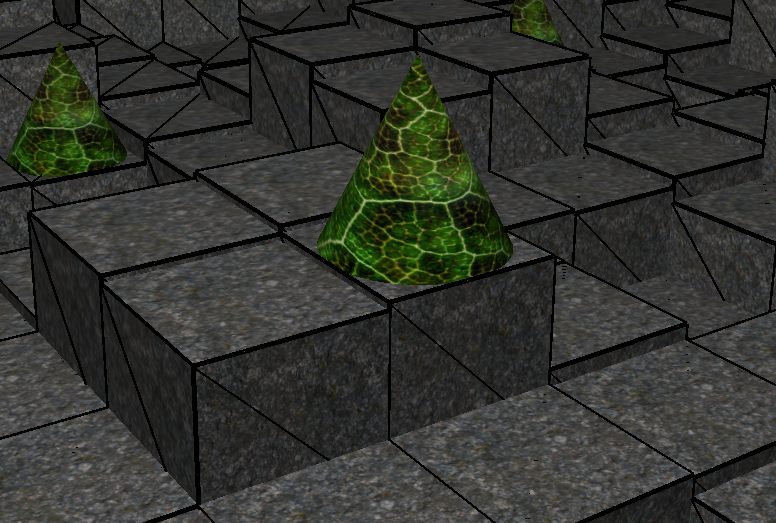
\includegraphics[scale=0.288]{wmode1.png}
    \caption{Nur Wireframes der Würfel}
\end{figure}
\end{minipage}
\begin{minipage}{0.5\textwidth}
\begin{figure}[H]
    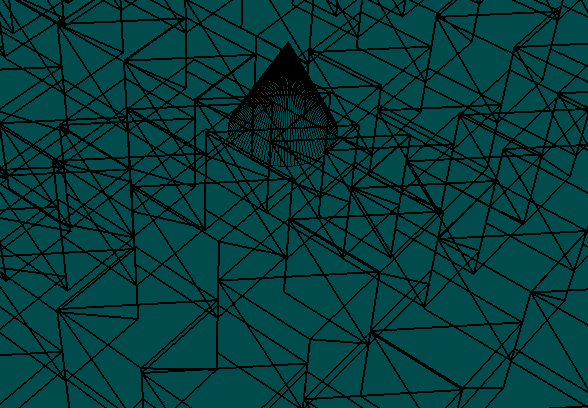
\includegraphics[scale=0.370]{wmode2.png}
    \caption{Ausschließlich Wireframes}
\end{figure}
\end{minipage}
\begin{minipage}{0.5\textwidth}
\begin{figure}[H]
    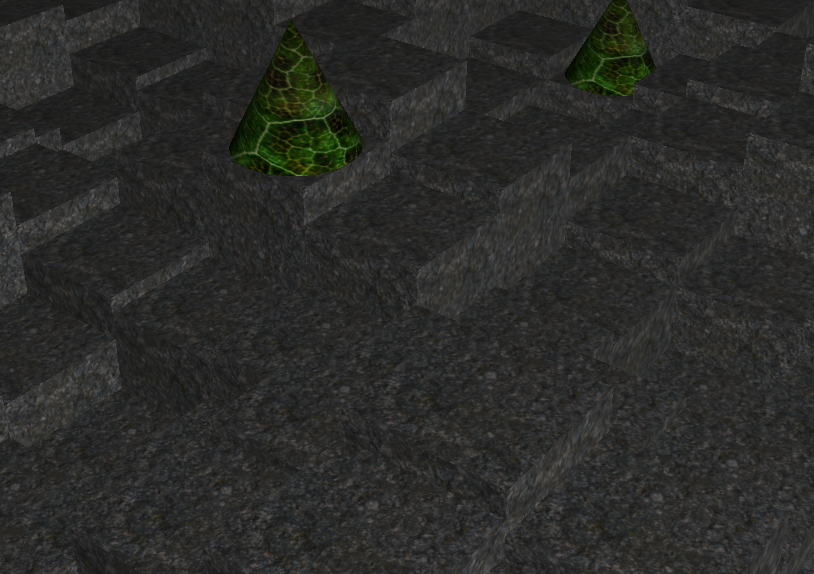
\includegraphics[scale=0.274]{wmode3.png}
    \caption{keine Wireframes}
\end{figure}
\end{minipage}
\begin{minipage}{0.5\textwidth}
\begin{figure}[H]
    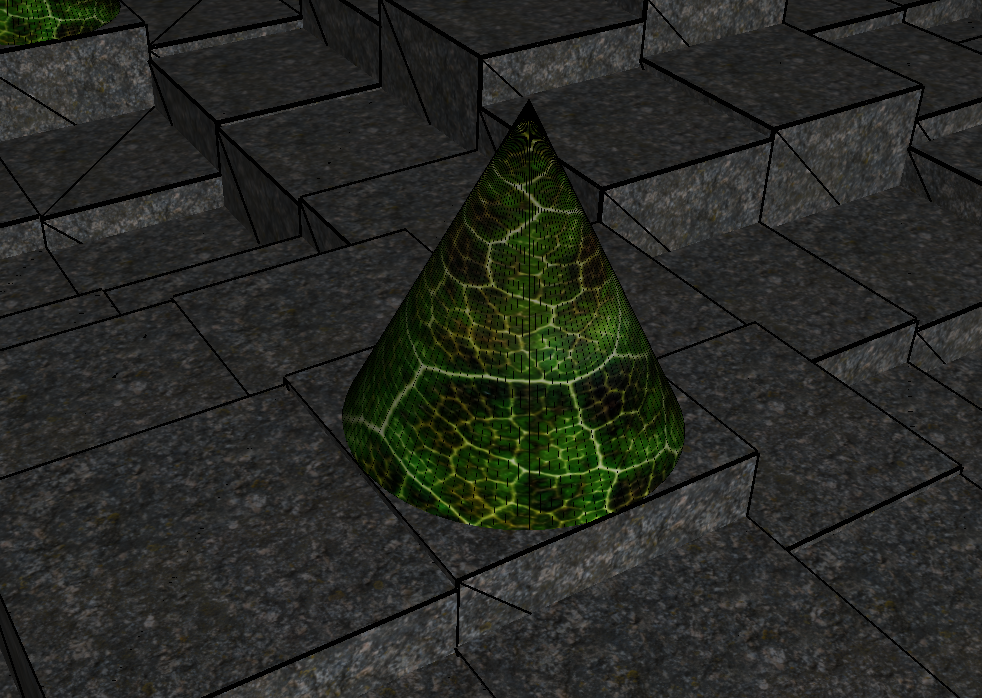
\includegraphics[scale=0.225]{wmode4.png}
    \caption{Alle Wireframes}
\end{figure}
\end{minipage}
\begin{figure}[H]
    \centering
    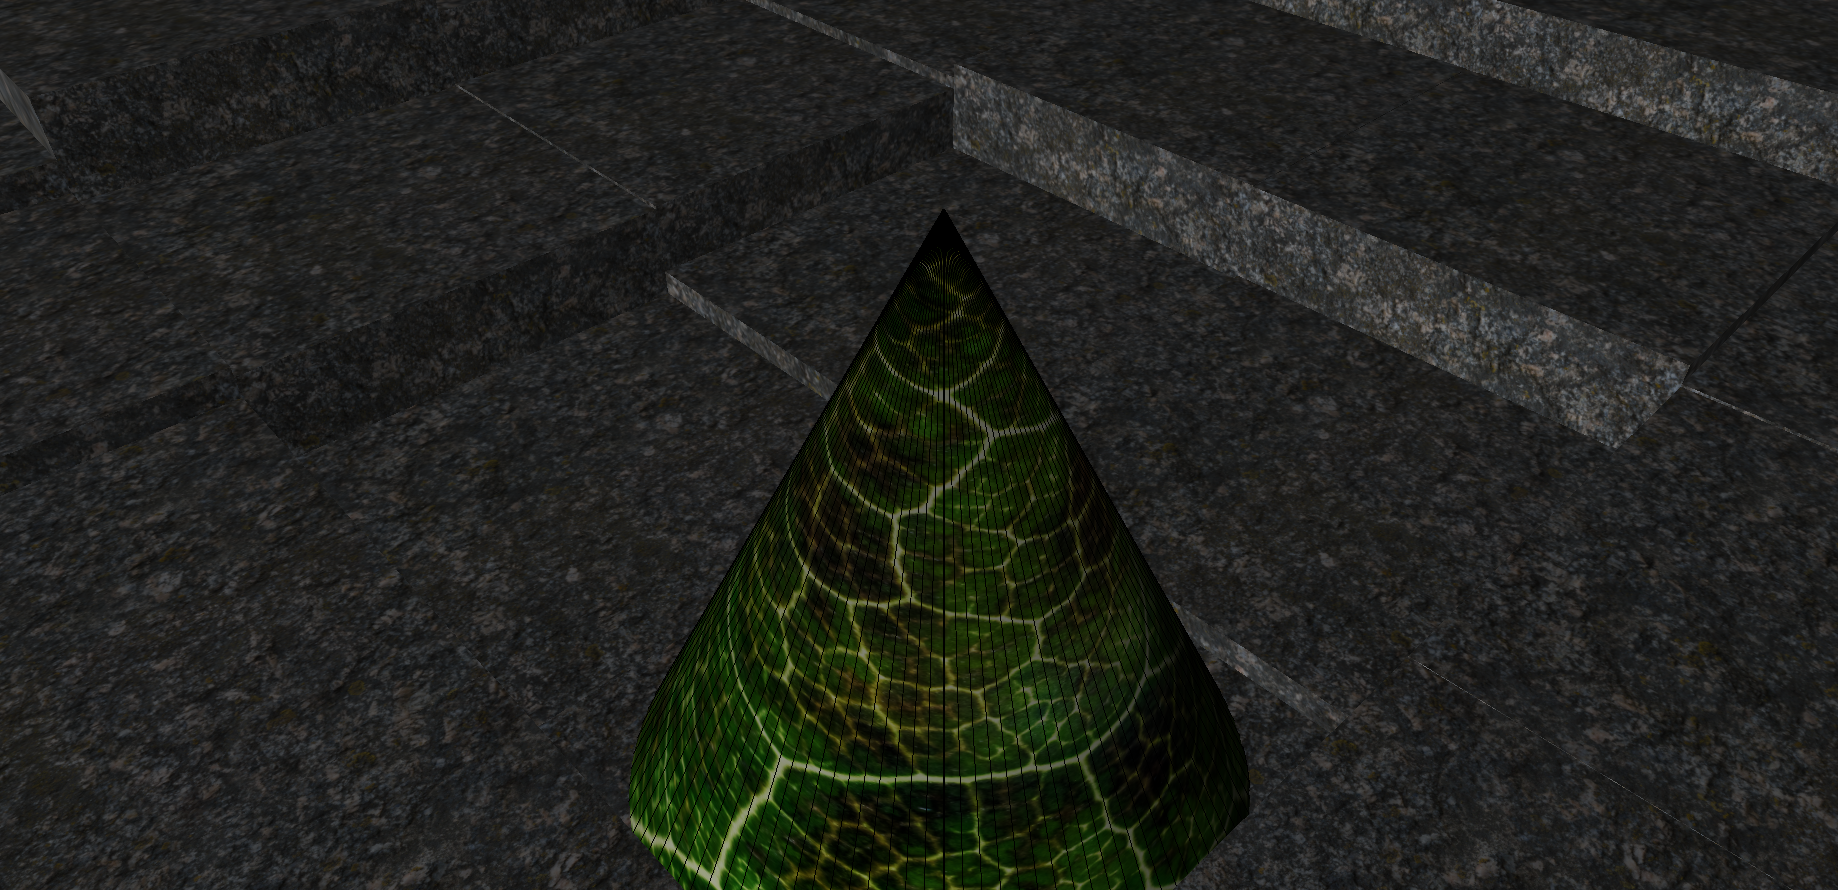
\includegraphics[scale=0.15]{wmode5.png}
    \caption{Nur Wireframes der Kegel}
\end{figure}

\subsection{OpenGL Optionen}
\subsubsection{Tiefentest}
Durch Betätigung der Taste \say{\textit{1}} lässt sich der Tiefentest (GL\_DEPTH\_TEST)
an- bzw. ausschalten.
\begin{minipage}{0.5\textwidth}
\begin{figure}[H]
    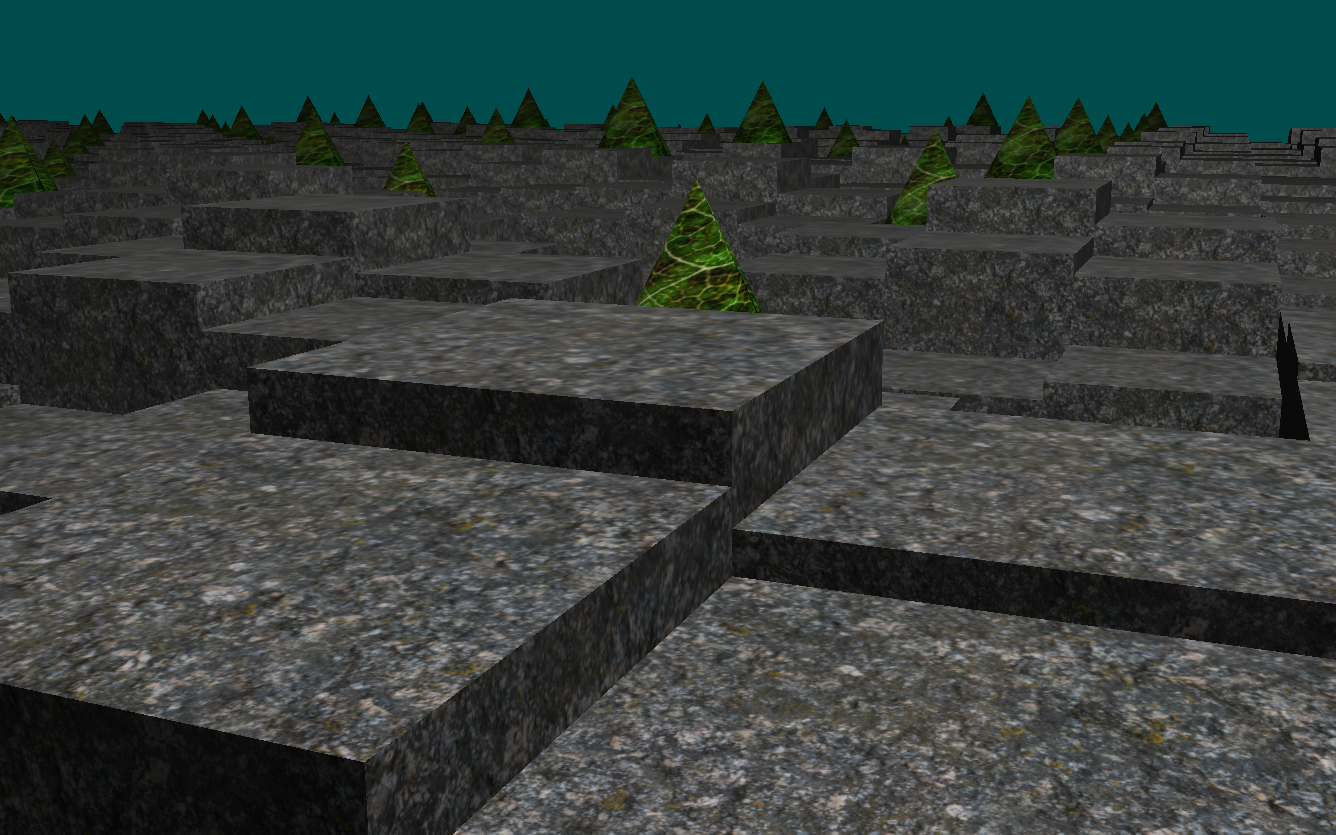
\includegraphics[scale=0.152]{omode1.png}
    \caption{Tiefentest Angeschaltet}
\end{figure}
\end{minipage}
\begin{minipage}{0.5\textwidth}
\begin{figure}[H]
    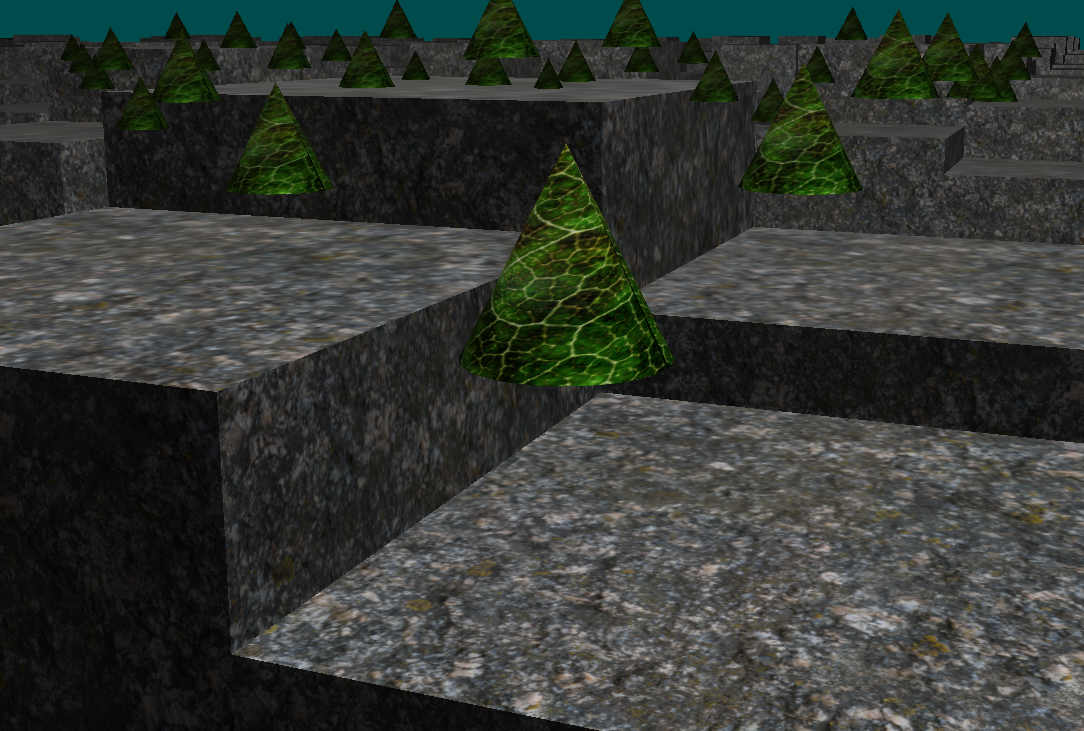
\includegraphics[scale=0.178]{omode2.png}
    \caption{Tiefentest Ausgeschaltet}
\end{figure}
\end{minipage}
\subsubsection{Face Culling}
Durch Betätigung der Taste \say{\textit{2}} lässt sich Face Culling (GL\_CULL\_FACE)
an- bzw. ausschalten. Dabei ist es wichtig das der Tiefentest ausgeschaltet ist ansonsten wird der
Effekt lediglich durch Performance Veränderungen bemerkbar.\\
\begin{minipage}{0.5\textwidth}
\begin{figure}[H]
    \centering
    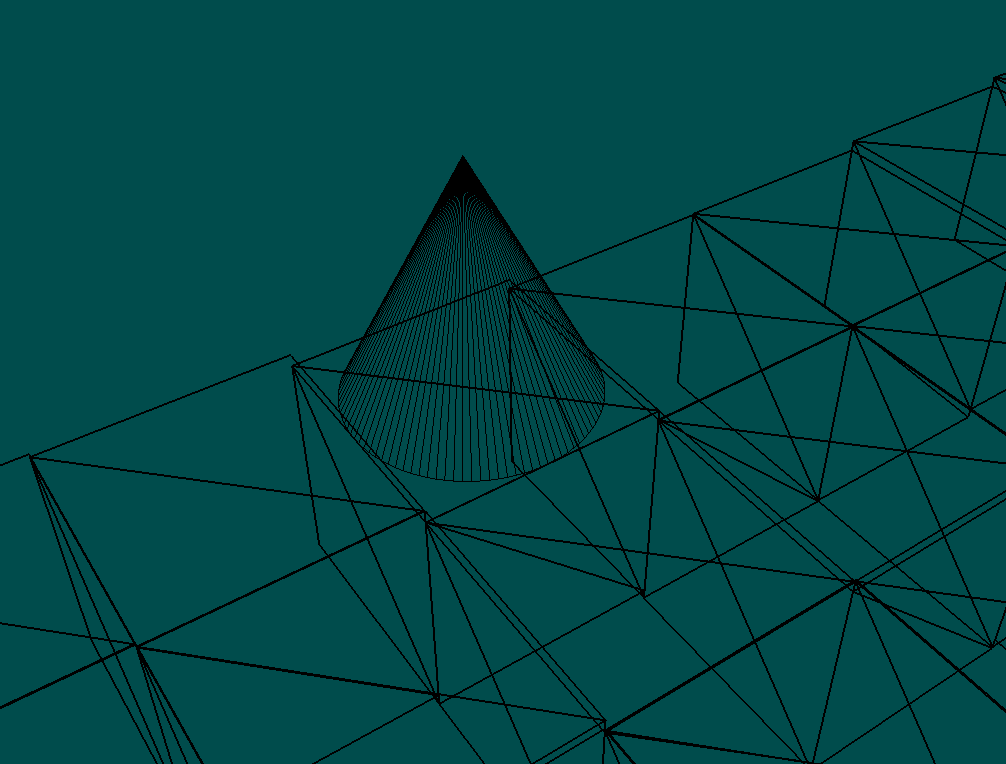
\includegraphics[scale=0.18]{omode3.png}
    \caption{Face Culling Angeschaltet}
\end{figure}
\end{minipage}
\begin{minipage}{0.5\textwidth}
\begin{figure}[H]
    \centering
    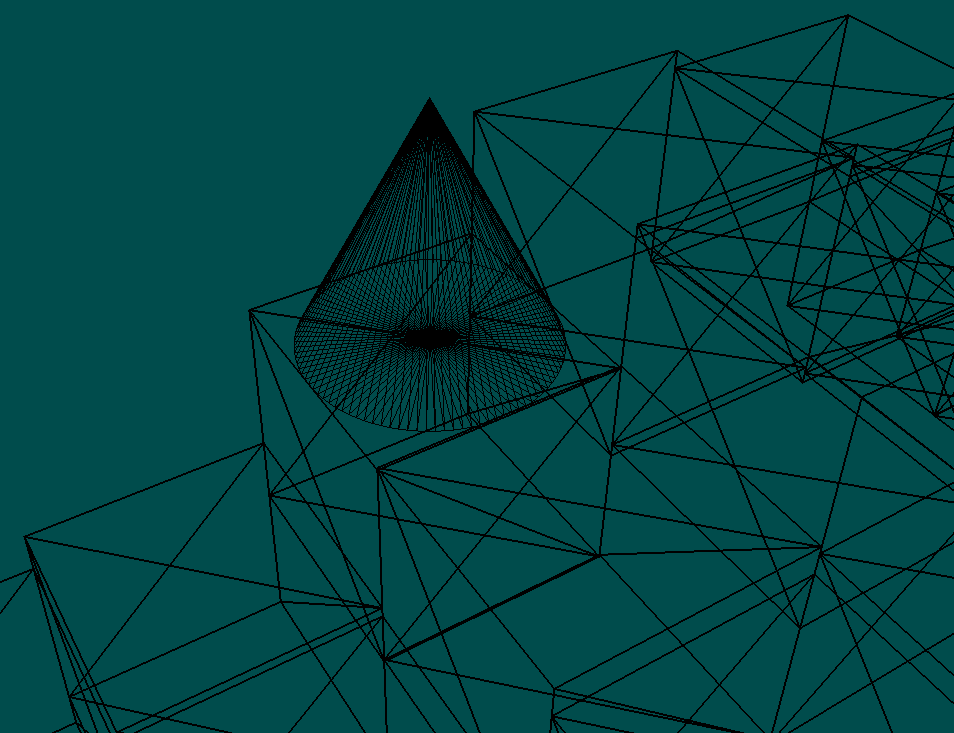
\includegraphics[scale=0.19]{omode4.png}
    \caption{Face Culling Ausgeschaltet}
\end{figure}
\end{minipage}

\subsection{Übersicht}
\begin{minipage}{0.56\textwidth}
\begin{table}[H]
\begin{tabular}{|l|l|}
\hline
\textit{\textbf{Taste}} & \textit{\textbf{Aktion}}                  \\ \hline
\textbf{w}              & nach vorne bewegen                        \\ \hline
\textbf{a}              & nach links bewegen                        \\ \hline
\textbf{s}              & nach hinten bewegen                       \\ \hline
\textbf{d}              & nach rechts bewegen                       \\ \hline
\textbf{e}              & nach oben bewegen                         \\ \hline
\textbf{q}              & nach unten bewegen                        \\ \hline
\textbf{c}              & wechsel der Lichtfarbe                    \\ \hline
\textbf{m}              & wechsel der Wirframe-Modien               \\ \hline
\textbf{l}              & wechsel der Art der Lichtquelle           \\ \hline
\textbf{v}              & wechsel zwischen einem und vier Viewports \\ \hline
\textbf{1}              & Tiefentest An- bzw. Ausschalten           \\ \hline
\textbf{2}              & Face Culling An- bzw. Ausschalten         \\ \hline
\end{tabular}
\end{table}
\end{minipage}
\begin{minipage}[b]{0.3\textwidth}
\begin{table}[H]
\begin{tabular}{|l|l|}
\hline
\textit{\textbf{Mausbewegung}} & \textit{\textbf{Aktion}} \\ \hline
\textbf{nach links}            & drehung nach links       \\ \hline
\textbf{nach rechts}           & drehung nach rechts      \\ \hline
\textbf{nach oben}             & neigung nach oben        \\ \hline
\textbf{nach unten}            & neigung nach unten       \\ \hline
\end{tabular}
\end{table}

\end{minipage}

\section{Dateien}
\subsection{C++ Quelltexte und Header Files}
\subsubsection{main.cpp}
In der Datei \say{main.cpp} befindet sich die Funktion \say{main}, welche als Einstiegspunkt für das Programm dient.
Des weiteren befinden sich in der Datei \say{main.cpp} unter anderem auch die Funktionen \say{init} welche
wichtige OpenGL zustände verändert sowie Shader, Texturen und die Objekte bereitstellt und \say{display}
welche 60 mal pro Sekunde aufgerufen wird und die Objekte zeichnet. 
\subsubsection{common.hpp}
In der Datei \say{common.hpp} werden globale Variablen auf die man von mehreren Dateien zugreifen können soll 
und einige enums sowie structs deklariert. Die Deklarationen betreffen programmweite Zustände und Inhalte die
von fast allen anderen Dateien benötigt werden. Initialisiert werden die globalen Variablen großteils in
der Datei \say{main.cpp}.
\subsubsection{shader.cpp \& shader.hpp}
In den Dateien \say{shader.cpp} und \say{shader.hpp} wird die Klasse \say{Shader} deklariert bzw. definiert.
Eine Instanz der Klasse besteht dabei aus einem Vertexshader und einem Fragmentshader.
Der Konstruktor der Klasse Shader liest und kompiliert die beiden Shaderdateien. Nach der erfolgreichen
Erstellung eines Shaderobjektes stellt die Klasse Methoden zur Verfügung die das aktivieren des Shaders sowie 
das setzen von uniform Variablen ermöglicht.
\subsubsection{camera.cpp \& camera.hpp}
In den Dateien \say{camera.cpp} und \say{camera.hpp} wird die Klasse \say{Camera} deklariert bzw. definiert.
Sie besteht aus Vektoren und anderen Variablen welche die Kamera auszeichnen sowie Methoden die je nach 
Mausbewegung oder Tastaturevents die Positions- bzw. Richtungsvektoren der Kamera verändern. Die Methode
\say{getViewMatrix} berechnet dann unter Verwendung der Memberdaten eine View-Matrix welche vor dem Zeichnen
per uniform Variable an den Shader übergeben wird. Durch den Konstruktor lässt sich der Kamera eine Ausgangsposition
und die Ausgangsblickrichtung in Form von Vektoren übergeben.
\subsubsection{callback.cpp \& callback.hpp}
In den Dateien \say{callback.cpp} und \say{callback.hpp} werden einige Callback-Funktionen deklariert bzw. definiert. 
Diese werden dann in der main-Funktion der OpenGL Bibliothek übergeben. Die Funktionen beschreiben das Verhalten bei
Mausbewegung, Tastaturevents oder dem Verändern der Fenstergröße. Die Funktionen agieren dabei mit einer Instanz der Klasse
\say{Camera} oder mit den in \say{common.h} deklarierten und \say{main.cpp} initialisierten Einstellungen.
\subsubsection{objects.cpp \& objects.hpp}
In den Dateien \say{objects.cpp} und \say{objects.hpp} werden Funktionen zur Erzeugung und Anordnung von geometrischen
Objekten deklariert bzw. definiert. Zur Erzeugung gibt es jeweils eine Funktion für den Würfel und Kegel.
Dabei werden die Vertex-Koordinaten, Textur-Koordinaten, Indizes und die Normalenvektoren berechnet bzw. angegeben.
Die Inhalte werden anschließend in ein \say{Vertex Buffer Object} kopiert und die Vertex-Attribute entsprechend
der Anordnung der Daten definiert. Die Funktion zur Anordnung der Objekte wurde bereits im Punkt \ref{Vorgehensweise}
\say{Vorgehensweise} auf Seite \pageref{Vorgehensweise}
beschrieben.
\subsubsection{textures.cpp \& textures.hpp}
Die Dateien \say{textures.cpp} und \say{textures.hpp} deklarieren bzw. definieren Funktionen die Texturen für den
Würfel und den Kegel laden und in Textur-Buffern speichert.

\subsection{Vertexshader}
\subsubsection{model\_shader.vs}
Der Vertexshader \say{model\_shader.vs} berechnet die Positionen der Vertices mithilfe einer View-,
Projection- und Model-Matrix. Diese Matrizen werden dem Shaderprogramm über uniform Variablen übergeben.
Des weiteren reicht der Vertexshader dem Fragmentshader Informationen über Farbe, Textur und Normalenvektoren weiter.
\subsubsection{instanced\_shader.vs}
Der Vertexshader \say{instanced\_shader.vs} unterscheidet sich dem Vertexshader \say{model\_shader.vs} nur in zwei Punkten.
Statt der Verwendung einer Model-Matrix die per uniform Variable definiert wird, werden hier auf verschiedene Instanzen,
die sich in einem Puffer befinden, zugegriffen. Im \say{instanced\_shader.vs} wird zusätzlich noch dem Fragmentshader 
die Position des Fragmentes übergeben.
\subsection{Fragmentshader}
\subsubsection{positional\_light.fs}
Im Fragmentshader \say{positional\_light.fs} wird die Farbe eines Fragmentes unter Verwendung der Farbe,
Textur, Fragment-Position und Normalenvektoren des Objektes sowie der Farbe und Position der Lichtquelle als auch 
der Position der Kamera berechnet. Mit diesen Daten kann dann die diffuse Veränderung des Lichtes (Änderung 
der Farbe durch den Winkel zwischen Objekt und Lichtquelle), die Dämpfung des Lichtes (Je weiter ein Fragment entfernt
von der Lichtquelle ist desto höher die Dämpfung) und die spiegelnde Reflexion (Wenn der Winkel von Lichtquelle zu Fragment
Ähnlich dem von Lichtquelle zu Kamera ist, entstehen helle Flecken) berechnet werden mit denen sich dann der gesamtwert
eines Fragmentes ermitteln lässt.
\subsubsection{light\_cube.fs}
Der Fragmentshader \say{light\_cube.fs} soll lediglich dem Würfel der die Lichtquelle darstellt seine Farbe geben.
Damit es so aussieht als wenn von dem Würfel Licht ausgeht, wird die Farbe der Fragmente auf die Farbe der Lichtquelle
gesetzt welche als uniform Variable dem Shaderprogramm übergeben wird.
\subsubsection{flashlight.fs}
Der Fragmentshader \say{flashlight.fs} ähnelt dem Fragmentshader \say{positional\_light.fs}. Diesmal werden allerdings
noch zwei weitere uniform Variablen übergeben. Dabei handelt es sich um zwei öffnungswinkel die den Lichtkegel der
Taschenlampe definieren. Der erste definiert den inneren Öffnungswinkel, der andere den äußeren. Fragmente die
im durch den inneren Winkel entstehenden Kegel liegen werden nicht abgeschwächt, Fragmente die außerhalb des durch
den äußeren Winkel enstehenden Kegels liegen werden dunkel (bis auf das Ambiente Licht). Zwischen den beiden Kegeln
entsteht ein helligkeitsverlauf.

\subsection{Texturen}
\subsubsection{cube1.jpg}
Die Datei \say{cube1.jpg} ist ein hochaufgelöstes Bild einer art Felswand welches ich als Textur für alle Seiten
des Würfels verwende. Gefunden habe ich das Bild auf der Webseite 3djungle.net auf der kostenlose und Open-Source
lizenzierte Texturen aufgelistet werden \cite{cube1}.
\subsubsection{cone1.jpg}
Die Datei \say{cone1.jpg} ist ein hochaufgelöste Makrofotografie eines Blattes welches ich als Textur für den
Kegel verwende. Gefunden habe ich das Bild auf der Webseite freestocktextures.com auf der
Texturen unter \say{Creative Commons Zero} Lizenz aufgelistet werden \cite{cone1}.

\section{Herausforderungen}
Bei der Entwicklung traten einige Herausforderungen und Probleme auf.
Einige dieser möchte ich im Folgenden weiter ausführen.
\subsection{Optimierung}
Durch die Entscheidung sehr viele Objekte zu zeichnen stellte sich mir die Frage in inwiefern ich das ganze
Optimieren kann bzw. muss.
Nach einiger Recherche entschloss ich mich dazu zwei Optimierungsmaßnahmen zu unternehmen.\par\medskip

Die erste Maßnahme war das verwenden von \say{Face Culling}. Die die dafür Notwendigen Implementierungs Veränderungen waren 
dabei sehr gering da ich bei der Implementierung der Funktionen für die Erzeugung der geometrischen Objekte bereits
auf die Reihenfolge der Vertices geachtet hatte. Durch das verwenden von \say{Face Culling} werden nur sichtbare
Flächen gerendert. Zum Beispiel können bei einem Würfel maximal drei Seiten gleichzeitig betrachtet werden.
Bei 10000 Würfeln erspart man sich in dem Falle also das rendern von 60000 Quadraten also 120000 Dreiecken.
Die resultierende Perfomance Veränderung kann durch Betrachtung der Grafikkarten Auslastung beim
Ein- und Ausschalten von \say{Face Culling} (Taste \textit{2}) betrachtet werden.\par\medskip

Die zweite und weitaus bedeutsamere Maßnahme war das verwenden von instanziiertem Zeichnen.
Die \say{draw}-Funktionen von OpenGL haben bekanntlich einen nicht zu geringen Overhead. Ohne die Verwendung
von instanziiertem Zeichnen sind 10400 aufrufe dieser Funktion pro Bild, bei 60 Bildern pro Sekunde 624000 Aufrufe
pro Sekunde, notwendig. Beim verwenden von instanziiertem Zeichnen werden die Model-Matrizen alle z.B. Würfel mit
einmal der Grafikkarte übergeben. Anschließend können alle Objekte dieses Types mit einem einzigem Aufruf einer
\say{draw}-Funktion gezeichnet werden. Pro Bild sind also nur 2 statt 10400 und somit pro Sekunde 120 statt 624000,
Aufrufe der \say{draw}-Funktion notwendig.

\subsection{Problem}
Beim Versuch ein Globales Objekt meiner Klasse \say{Shader} zu erzeugen, erhielt ich nach erfolgreichem Compilieren
einen Speicherzugriffsfehler. Nachdem ich keine offensichtlichen Fehler finden konnte, entschied ich mich einen
Debugger zu verwenden um den Fehler zu lokalisieren. Dieser zeigte mir zunächst das der Fehler in einer Nvidia
Bibliothek, also ausserhalb meines Programmes auftrat. Durch das Betrachten des Stacktraces entdeckte ich die
Zeile die das Problem verursachte. Es handelte sich dabei um die Zeile \say{GLuint vertex=glCreateShader(GL\_VERTEX\_SHADER);}
die sich im Konstruktor der Klasse \say{Shader} befand. Dies verwirrte mich zunächst sehr. Das Internet war mir 
in dem Moment auch keine große Hilfe. Nach einiger Zeit wurde mir das Problem klar. Globale Variablen werden
initialisiert bevor die \say{main}-Funktion ausgeführt wird. Dies hatte zur folge das OpenGL Befehle vor notwendigen
Initialisierungen ausgeführt wurden und somit den Fehler verursachten.\par\medskip

Behoben habe ich den Fehler indem ich lediglich einen Pointer vom Typ der Klasse \say{Shader} Global deklariert habe
und erst später, nach den notwendigen Initialisierungen, auf dem Heap ein Objekt dieser Klasse erzeugt und der
globalen Variable zugewiesen habe.

\subsection{Maus Cursor}
\newpage
\printbibliography
\end{document}
